\section[Desenvolvimento do Projeto]{Desenvolvimento do Projeto}

\subsection{Repositório do Código Fonte do Projeto}
Nossa estrutura de versionamento seguiu uma lógica similar aos projetos passados, sendo distribuída em três repositórios principais: \textit{Wiki}, \textit{backend} e \textit{frontend}. Cada um deles teve um papel bem definido dentro do ciclo de desenvolvimento:

O repositório \textit{Wiki} concentrou a documentação geral do projeto, servindo de base para o registro de decisões, requisitos, modelos e materiais de apoio. O conteúdo está disponível em: \url{https://tools.ages.pucrs.br/weconecta-plataforma-digital-para-question-rios-de-sa-de/wiki/-/wikis/home}.

O repositório \textit{backend} armazenou o código responsável pela API, pela lógica de negócio e pelas integrações do sistema. O código está disponível em: \url{https://tools.ages.pucrs.br/weconecta-plataforma-digital-para-question-rios-de-sa-de/backend}.

Por fim, o repositório \textit{frontend} manteve o código da interface do usuário, incluindo telas, componentes e lógica de interação. O código está disponível em: \url{https://tools.ages.pucrs.br/weconecta-plataforma-digital-para-question-rios-de-sa-de/frontend}.



\subsection{Banco de Dados Utilizado}
O projeto WeConecta utilizou o PostgreSQL como sistema gerenciador de banco de dados. Conforme registrado na \textit{Wiki} do projeto, a escolha considerou a robustez do sistema, sua consistência transacional, o suporte nativo a JSON e sua adequação a modelos que combinam dados relacionais e estruturas em JSON. Essas características eram pertinentes ao projeto porque o sistema precisava manter relações entre usuários, questionários, elementos e respostas, além de representar o fluxo configurável de cada questionário.

O esquema lógico inicial, proposto pelos AGES II e apresentado na Figura~\ref{fig:db-logical-wecon}, organizava o domínio em torno das entidades de usuário, questionário, mensagem, alternativa e resposta. Entidades associativas também representavam a colaboração de usuários nos questionários e as conexões entre as mensagens que compunham cada fluxo.

\begin{figure}[H]
  \centering
  \small
  \caption{Diagrama lógico inicial do banco de dados do projeto WeConecta}
  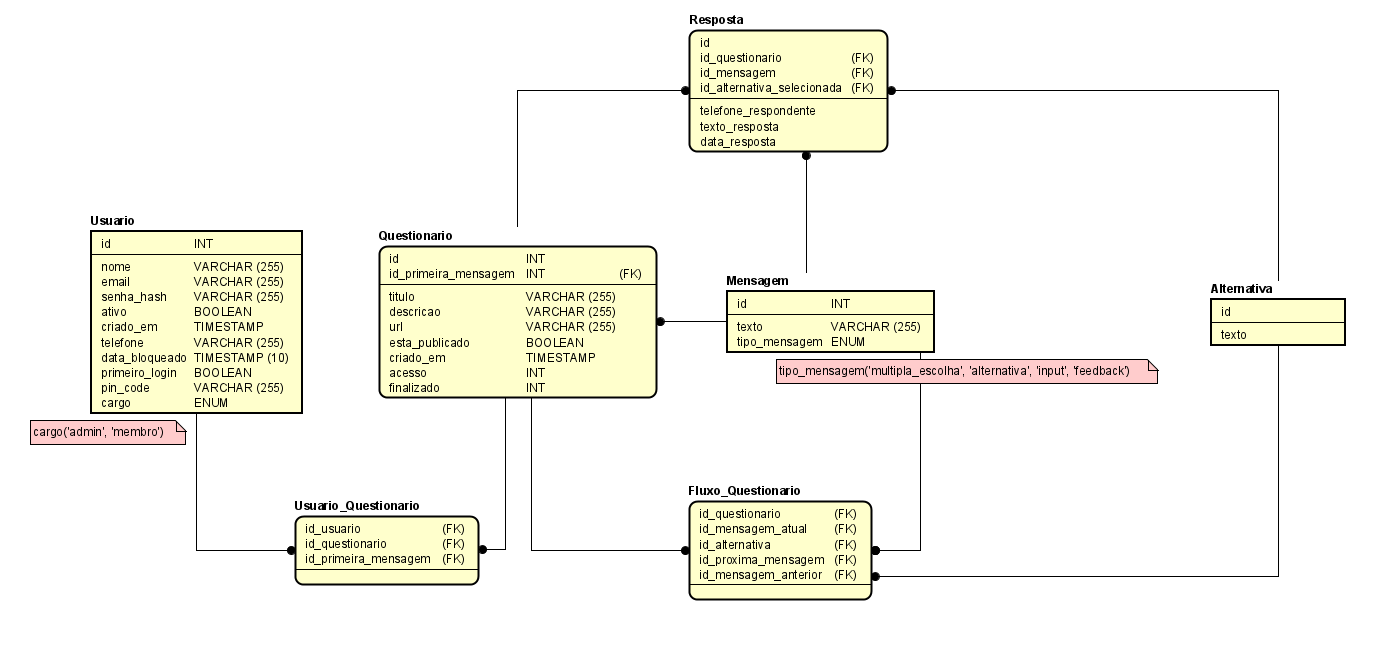
\includegraphics[width=1\linewidth]{conteudo//4 - ages III//conteudo//figures/banco-esquema-lógico.png}
  Fonte: \textit{Wiki} do projeto
  \label{fig:db-logical-wecon}
\end{figure}

À medida que o desenvolvimento avançou e o time recebeu retornos dos \textit{stakeholders}, o modelo passou por sucessivas revisões. Nos esquemas finais, as mensagens e os demais componentes dos questionários foram consolidados como elementos de questionário, enquanto suas possíveis opções passaram a ser representadas separadamente. O modelo conceitual foi elaborado com o brModelo, e o modelo lógico, com o dbdiagram.io. Os resultados são apresentados nas Figuras~\ref{fig:db-concept-wecon} e~\ref{fig:db-logic-wecon}, respectivamente.
\begin{figure}[H]
  \centering
  \small
  \caption{Diagrama conceitual final do banco de dados do projeto WeConecta}
  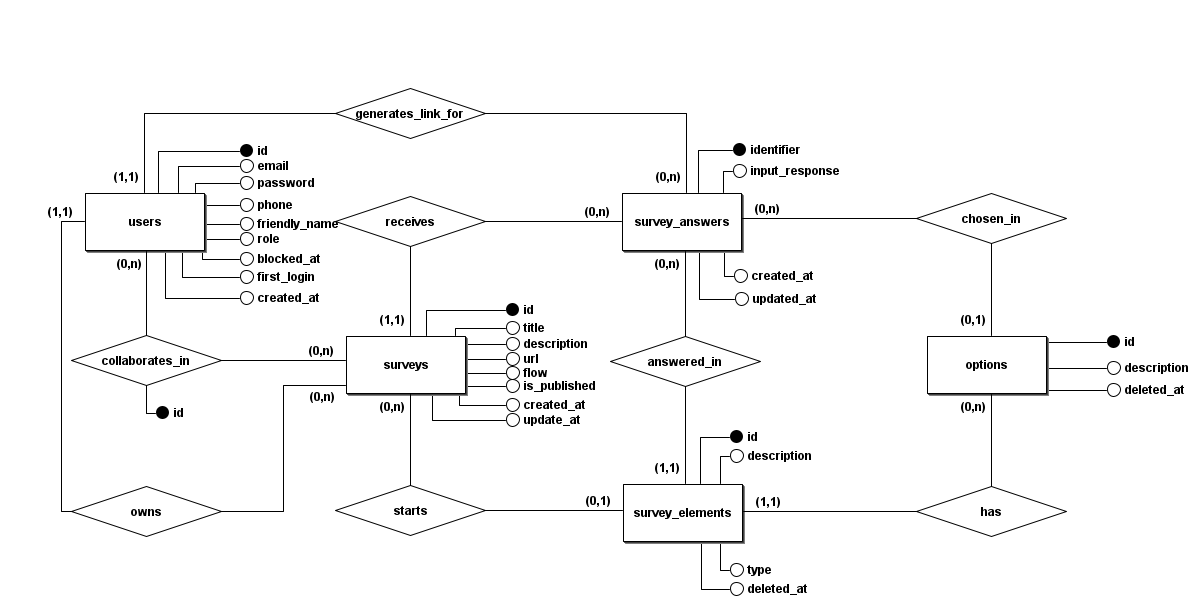
\includegraphics[width=1\linewidth]{conteudo//4 - ages III//conteudo//figures/banco-final-conceitual.png}
  Fonte: \textit{Wiki} do projeto
  \label{fig:db-concept-wecon}
\end{figure}

\begin{figure}[H]
  \centering
  \small
  \caption{Diagrama lógico final do banco de dados do projeto WeConecta}
  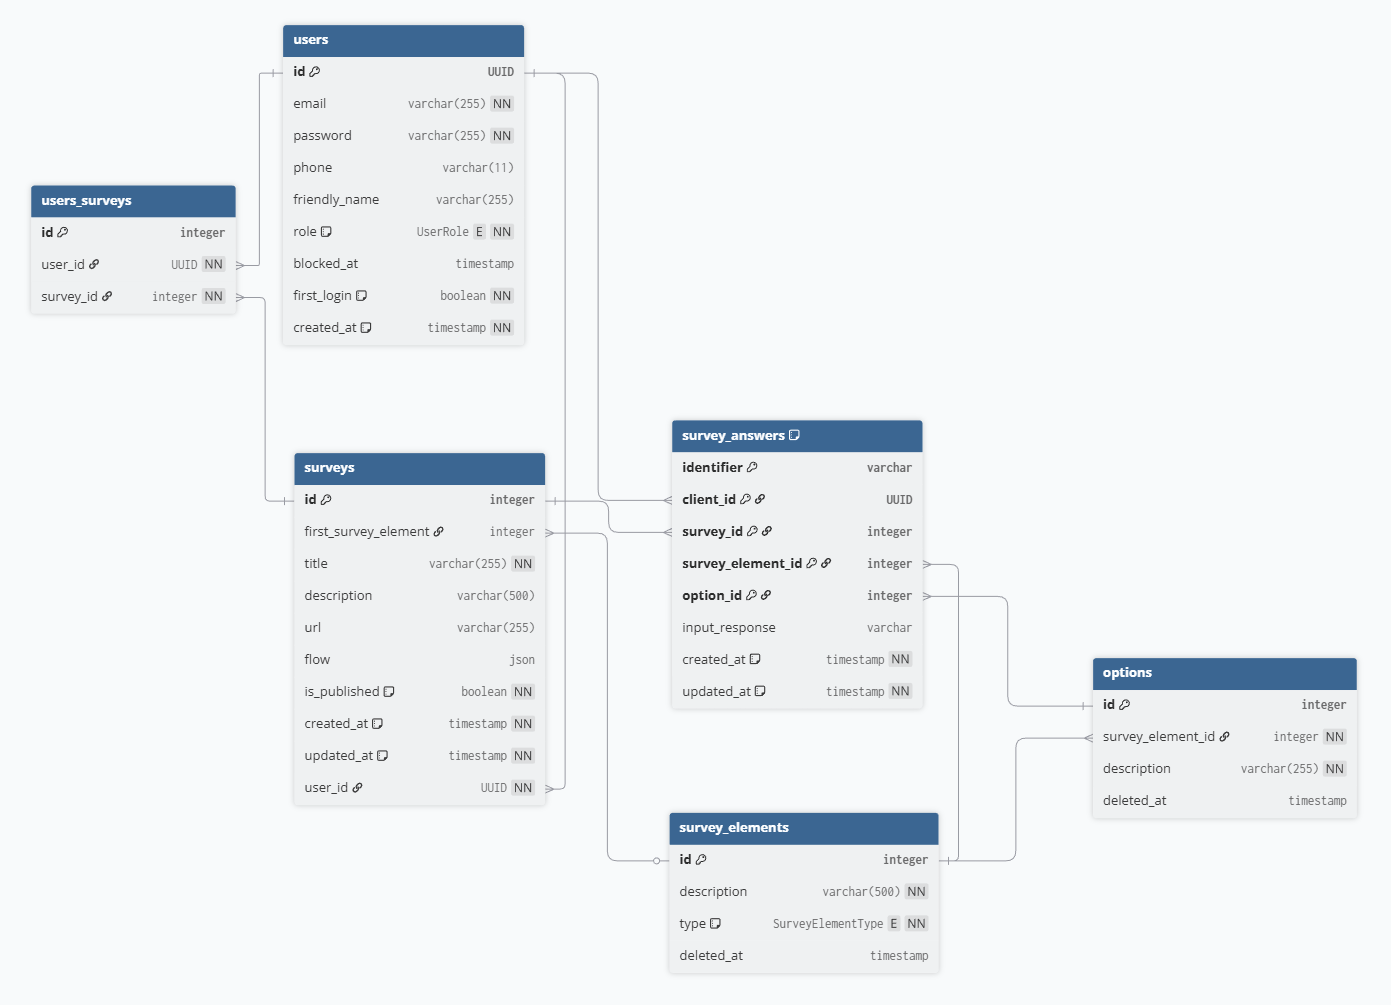
\includegraphics[width=1\linewidth]{conteudo//4 - ages III//conteudo//figures/banco-final-lógico2.png}
  Fonte: \textit{Wiki} do projeto
  \label{fig:db-logic-wecon}
\end{figure}

O modelo final ficou organizado em seis tabelas principais. A tabela \textit{users} armazena os usuários e seus papéis no sistema, enquanto \textit{surveys} reúne os questionários, seus metadados, o responsável por sua criação e a estrutura do fluxo em JSON. A relação de colaboração entre usuários e questionários é mantida por \textit{users\_surveys}. As tabelas \textit{survey\_elements} e \textit{options} representam, respectivamente, os elementos que compõem um questionário e as opções vinculadas a eles. Por fim, \textit{survey\_answers} associa as respostas ao questionário, ao elemento respondido e, quando aplicável, à opção escolhida, permitindo também o armazenamento de respostas textuais.

A documentação detalhada do banco de dados está disponível em: \url{https://tools.ages.pucrs.br/weconecta-plataforma-digital-para-question-rios-de-sa-de/wiki/-/wikis/banco_dados}.

\subsection{Arquitetura Utilizada}

A concepção inicial da arquitetura teve como foco a simplicidade, o custo e a fluidez operacional. Nessa configuração, o \textit{frontend} seria hospedado no AWS Amplify, a fim de facilitar o \textit{deploy} e a \ac{cicd}. Já o \textit{backend} residiria em uma instância EC2 dentro de uma \textit{subnet} privada, containerizada via Docker.
A comunicação entre o cliente e o \textit{backend} seria mediada pelo AWS API Gateway, que direcionaria as requisições para nossa API. Essa API se comunicaria diretamente com a instância de banco de dados dentro da mesma VPC, mantendo a segurança e o isolamento da infraestrutura. Essa idealização é apresentada na Figura~\ref{fig:infra-init}.

\begin{figure}[H]
  \centering
  \small
  \caption{Diagrama inicial da infraestrutura \textit{cloud} do projeto WeConecta}
  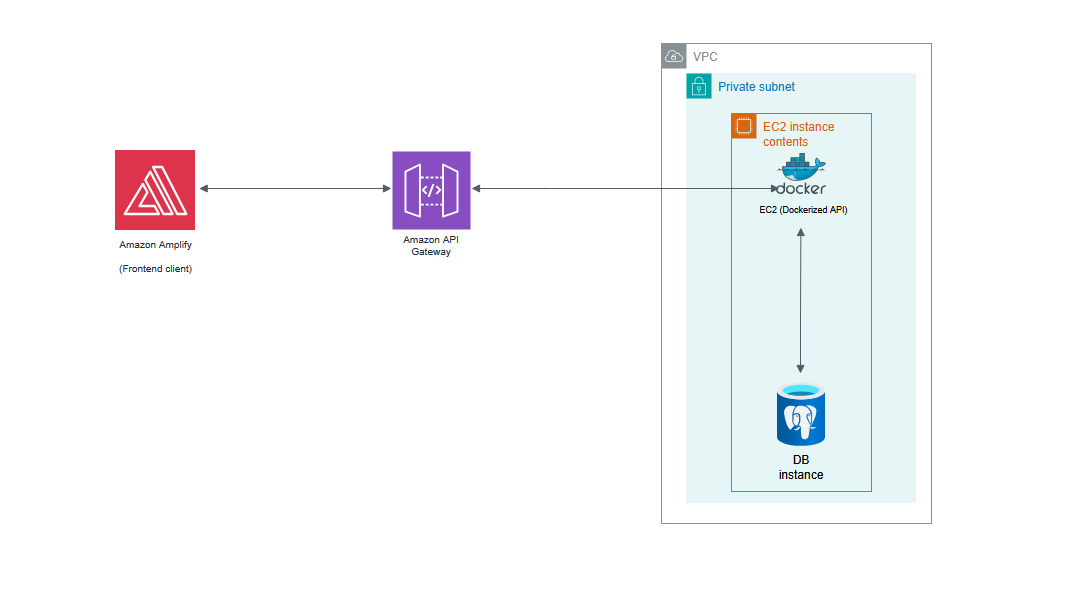
\includegraphics[width=1\linewidth]{conteudo//4 - ages III//conteudo//figures/init-infra.png}
  Fonte: \textit{Wiki} do projeto
  \label{fig:infra-init}
\end{figure}

Porém, com o avanço do projeto, surgiram alguns contratempos relacionados à AWS. Isso nos levou à nova estrutura apresentada na Figura~\ref{fig:final-infra}.
A estrutura final posiciona a instância EC2 em uma \textit{subnet} pública, de forma que o \textit{frontend} se comunica diretamente com o \textit{backend}, sem a mediação do API Gateway. O banco de dados continuou hospedado na mesma EC2 que a API, e o \textit{frontend} também não sofreu alterações quanto ao uso do serviço Amplify para fins de \textit{deploy}.

\begin{figure}[H]
  \centering
  \small
  \caption{Diagrama final da infraestrutura \textit{cloud} do projeto WeConecta}
  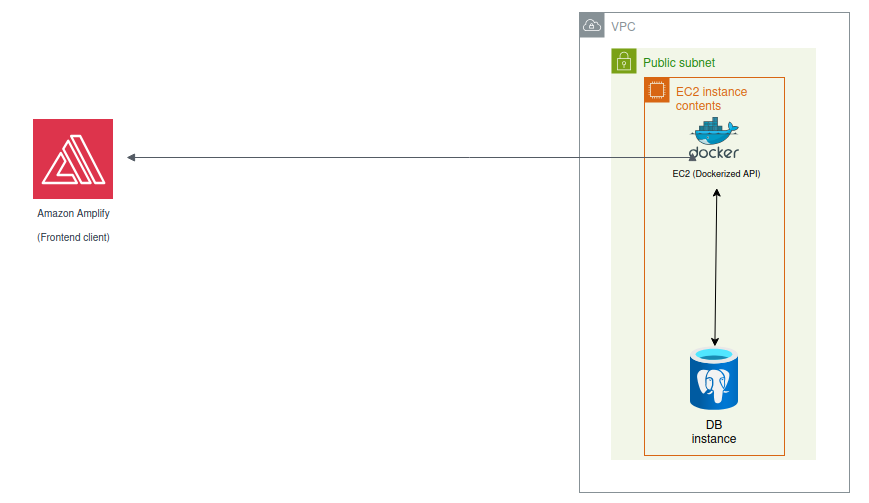
\includegraphics[width=1\linewidth]{conteudo//4 - ages III//conteudo//figures/final-infra.png}
  Fonte: \textit{Wiki} do projeto
  \label{fig:final-infra}
\end{figure}

\subsection{Protótipos das Telas Desenvolvidas}
As telas desenvolvidas pelo time são apresentadas nas Figuras~\ref{fig:screen1} a~\ref{fig:screen10}.

\begin{figure}[H]
  \centering
  \small
  \caption{Dashboard (Home) – Todos os usuários}
  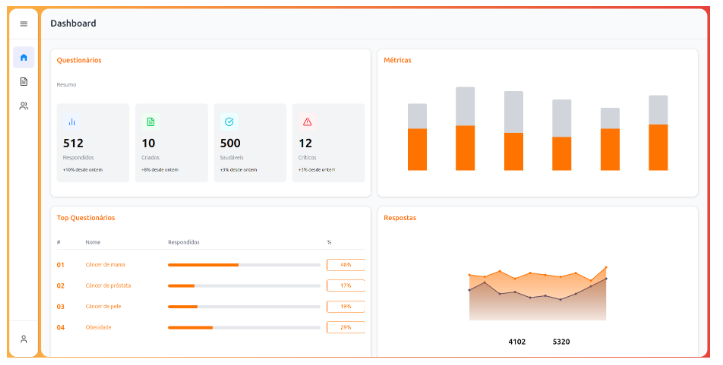
\includegraphics[width=1\linewidth]{conteudo//4 - ages III//conteudo//figures/dashboard-home.png}
  Fonte: Autor
  \label{fig:screen1}
\end{figure}

\begin{figure}[H]
  \centering
  \small
  \caption{Visualização dos questionários – Todos os usuários}
  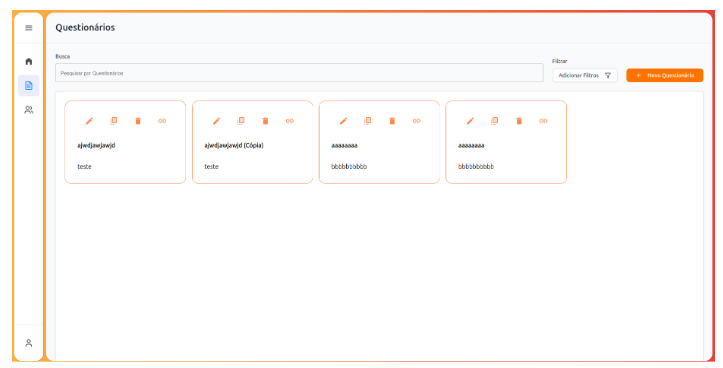
\includegraphics[width=1\linewidth]{conteudo//4 - ages III//conteudo//figures/survey-all-users.png}
  Fonte: Autor
  \label{fig:screen2}
\end{figure}

\begin{figure}[H]
  \centering
  \small
  \caption{Sidebar}
  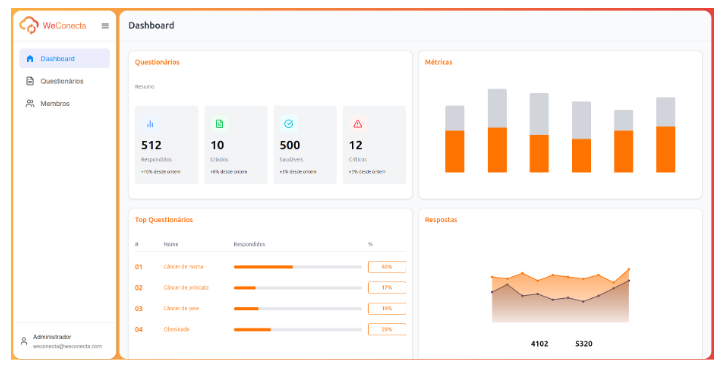
\includegraphics[width=1\linewidth]{conteudo//4 - ages III//conteudo//figures/sidebar-display.png}
  Fonte: Autor
  \label{fig:screen3}
\end{figure}

\begin{figure}[H]
  \centering
  \small
  \caption{Modal de Criação de Questionários – Administradores}
  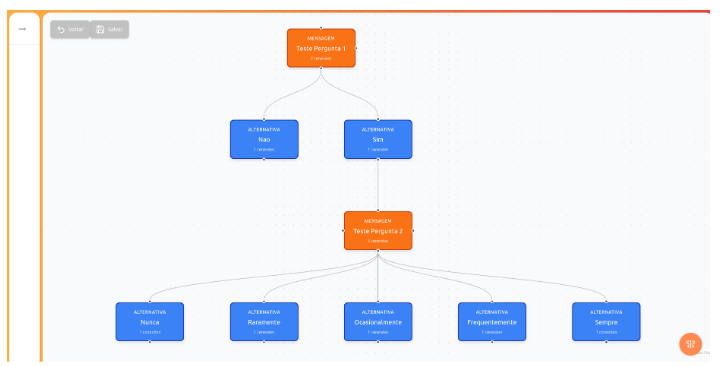
\includegraphics[width=1\linewidth]{conteudo//4 - ages III//conteudo//figures/survey-flow-create-admin.png}
  Fonte: Autor
  \label{fig:screen4}
\end{figure}

\begin{figure}[H]
  \centering
  \small
  \caption{Tela de Criação do Fluxo de Questionário – Administradores}
  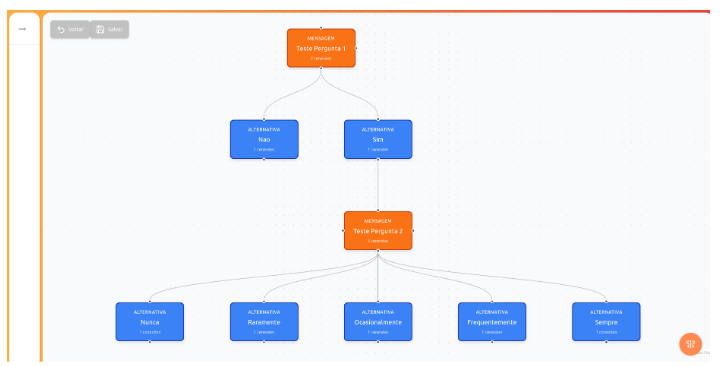
\includegraphics[width=1\linewidth]{conteudo//4 - ages III//conteudo//figures/survey-flow-create-admin.png}
  Fonte: Autor
  \label{fig:screen5}
\end{figure}

\begin{figure}[H]
  \centering
  \small
  \caption{Mensagem de Deleção de Conexão ou Nodo – Administradores}
  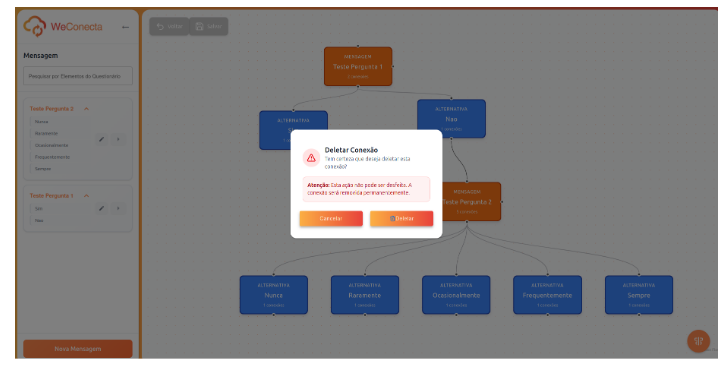
\includegraphics[width=1\linewidth]{conteudo//4 - ages III//conteudo//figures/delete-node-or-conn-survey.png}
  Fonte: Autor
  \label{fig:screen6}
\end{figure}

\begin{figure}[H]
  \centering
  \small
  \caption{Criação de Elementos do Questionário – Administradores}
  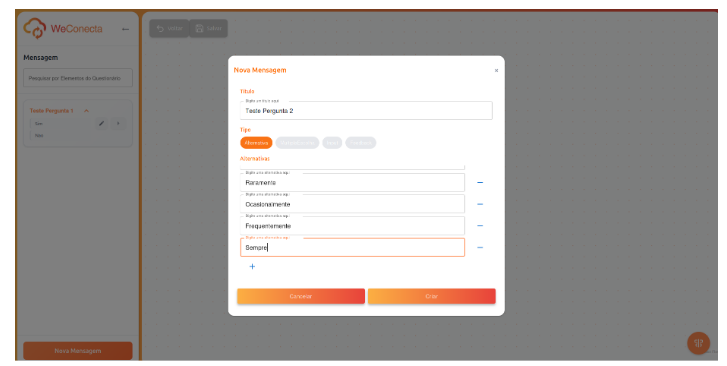
\includegraphics[width=1\linewidth]{conteudo//4 - ages III//conteudo//figures/create-survey-element.png}
  Fonte: Autor
  \label{fig:screen7}
\end{figure}

\begin{figure}[H]
  \centering
  \small
  \caption{Tela de Gerenciamento de Usuários – Administradores}
  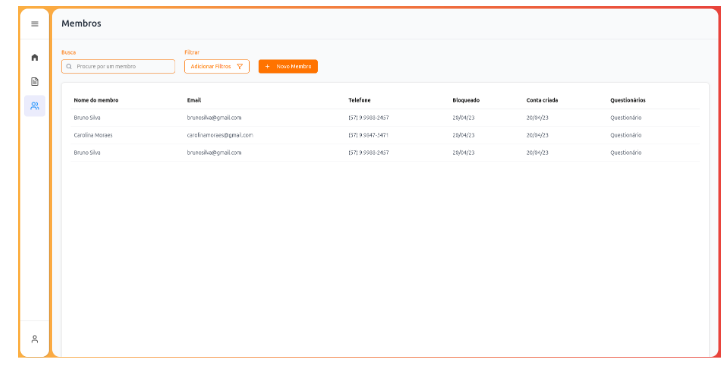
\includegraphics[width=1\linewidth]{conteudo//4 - ages III//conteudo//figures/manage-users.png}
  Fonte: Autor
  \label{fig:screen9}
\end{figure}

\begin{figure}[H]
  \centering
  \small
  \caption{Modal de Criação de Usuários – Administradores}
  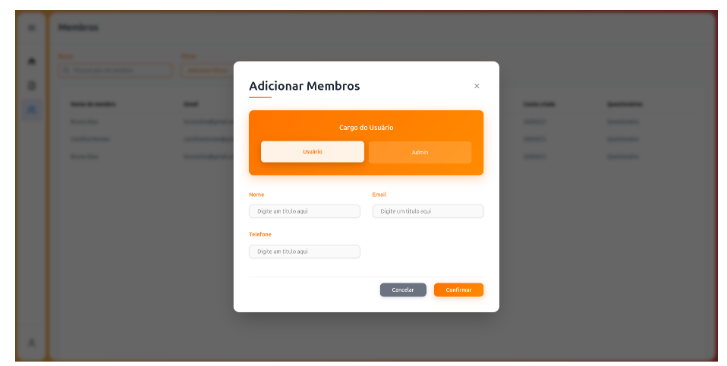
\includegraphics[width=1\linewidth]{conteudo//4 - ages III//conteudo//figures/create-user-manage-user.png}
  Fonte: Autor
  \label{fig:screen10}
\end{figure}


\subsection{Tecnologias Utilizadas}
A base do desenvolvimento concentrou-se na linguagem TypeScript, escolhida tanto para o lado do servidor quanto para a aplicação do usuário, permitindo padronização e consistência no \textit{onboarding} da equipe. O \textit{backend} foi construído com NestJS, adotado por sua arquitetura modular e opinativa. No \textit{frontend}, a escolha recaiu sobre o Next.js, que possibilitou a criação de interfaces dinâmicas de acordo com as sugestões e os requisitos dos \textit{stakeholders}. Para o armazenamento de dados, optou-se pelo SGBD PostgreSQL.

A infraestrutura foi sustentada principalmente por serviços da AWS, com uma instância EC2 dedicada à execução do \textit{backend} e do banco de dados. Já o AWS Amplify ficou responsável pelo fluxo de disponibilização do \textit{frontend}, em tese, facilitando atualizações e garantindo estabilidade. Complementando essa arquitetura, o GitLab CI foi utilizado para orquestrar \textit{pipelines} de integração contínua, permitindo automatizar tarefas como \textit{build}, testes e \textit{deploy}, além de garantir maior rastreabilidade durante o ciclo de desenvolvimento.
